\documentclass[a4paper,11pt]{article}
\usepackage{amsmath,amsthm,amsfonts,amssymb,amscd,amstext,vmargin,graphics,graphicx,tabularx,multicol} \usepackage[french]{babel}
\usepackage[utf8]{inputenc}  
\usepackage[T1]{fontenc} 
\usepackage[T1]{fontenc}
\usepackage{amsmath,amssymb}
\usepackage{pstricks-add,tikz,tkz-tab,variations}
\usepackage[autolanguage,np]{numprint} 
\usepackage{color}
\usepackage{ulem}

\setmarginsrb{1.5cm}{0.5cm}{1cm}{0.5cm}{0cm}{0cm}{0cm}{0cm} %Gauche, haut, droite, haut
\newcounter{numexo}
\newcommand{\exo}[1]{\stepcounter{numexo}\noindent{\bf Exercice~\thenumexo} : \marginpar{\hfill /#1}}
\reversemarginpar


\newcounter{enumtabi}
\newcounter{enumtaba}
\newcommand{\q}{\stepcounter{enumtabi} \theenumtabi.  }
\newcommand{\qa}{\stepcounter{enumtaba} (\alph{enumtaba}) }
\newcommand{\initq}{\setcounter{enumtabi}{0}}
\newcommand{\initqa}{\setcounter{enumtaba}{0}}

\newcommand{\be}{\begin{enumerate}}
\newcommand{\ee}{\end{enumerate}}
\newcommand{\bi}{\begin{itemize}}
\newcommand{\ei}{\end{itemize}}
\newcommand{\bp}{\begin{pspicture*}}
\newcommand{\ep}{\end{pspicture*}}
\newcommand{\bt}{\begin{tabular}}
\newcommand{\et}{\end{tabular}}
\renewcommand{\tabularxcolumn}[1]{>{\centering}m{#1}} %(colonne m{} centrée, au lieu de p par défault) 
\newcommand{\tnl}{\tabularnewline}

\newcommand{\trait}{\noindent \rule{\linewidth}{0.2mm}}
\newcommand{\hs}[1]{\hspace{#1}}
\newcommand{\vs}[1]{\vspace{#1}}

\newcommand{\N}{\mathbb{N}}
\newcommand{\Z}{\mathbb{Z}}
\newcommand{\R}{\mathbb{R}}
\newcommand{\C}{\mathbb{C}}
\newcommand{\Dcal}{\mathcal{D}}
\newcommand{\Ccal}{\mathcal{C}}
\newcommand{\mc}{\mathcal}

\newcommand{\vect}[1]{\overrightarrow{#1}}
\newcommand{\ds}{\displaystyle}
\newcommand{\eq}{\quad \Leftrightarrow \quad}
\newcommand{\vecti}{\vec{\imath}}
\newcommand{\vectj}{\vec{\jmath}}
\newcommand{\Oij}{(O;\vec{\imath}, \vec{\jmath})}
\newcommand{\OIJ}{(O;I,J)}

\newcommand{\bmul}[1]{\begin{multicols}{#1}}
\newcommand{\emul}{\end{multicols}}


\newcommand{\reponse}[1][1]{%
\multido{}{#1}{\makebox[\linewidth]{\rule[0pt]{0pt}{20pt}\dotfill}
}}

\newcommand{\titre}[5] 
% #1: titre #2: haut gauche #3: bas gauche #4: haut droite #5: bas droite
{
\noindent #2 \hfill #4 \\
#3 \hfill #5

\vspace{-1.6cm}

\begin{center}\rule{6cm}{0.5mm}\end{center}
\vspace{0.2cm}
\begin{center}{\large{\textbf{#1}}}\end{center}
\begin{center}\rule{6cm}{0.5mm}\end{center}
}



\begin{document}
\pagestyle{empty}
\titre{Contrôle type Brevet}{Nom}{Prénom}{Date}{Classe}


\vspace*{0.75cm}

\exo{2}

\q On donne l'expression $E = (3x +8)^{2} -2(x+1)$. \textbf{Développer} l'expression E.\\

\q On donne l'expression $L = (3x-11)(9-x)-(-5x+27)(9-x)$. \textbf{Factoriser} l'expression L.\\

\vspace*{0.5cm}

\exo{5} Résoudre les équations suivantes :

\bmul{2}


\qa $ -11 - 5x = - 76$\\


\qa $2-2x = 5x + 3$\\




\columnbreak




\qa $4x - 19 = 7x - 10 $\\


\qa $2(7 -2x) = -3(x -7)$\\








\emul





\exo{3} Résoudre les problèmes à l'aide des équations.\\

\initq \q Pierre et Nathalie possèdent ensemble 144 timbres de collection. Si Nathalie donnait deux timbres à Pierre, alors celui-ci en aurait deux fois plus qu'elle. Combien chaque enfant a-t-il de timbres actuellement ?\\


\q Un père dispose de 1 600 euros pour ses trois enfants. Il veut que l'aîné ait 200 euros de plus que le second et
que le second ait 100 euros de plus que le dernier. Comment fait-il cette répartition ?\\

\vspace*{0.5cm}

\exo{4.5}\\

La figure suivante est donnée à titre indicatif pour préciser la position des points A, B, C, D et E. \\
Les longueurs représentées ne le sont pas en vraie grandeur.\\
On donne CE = 5 m, CD = 12 m, CA = 18 m, CB = 7,5 m, AB = 19,5m. Les droites (AB) et(ED) sont parallèles.\\

\bmul{2}
\noindent \initq \q  Montrer que ED = 13 m.\\
\q  Montrer que le triangle CED est un triangle rectangle.\\
\q Déterminer un valeur arrondie au degré près de la mesure de l'angle DEC.\\

\columnbreak


\includegraphics[scale=1]{imagebrevet.eps} 


\emul


\exo{5.5}\\

Une maison est composée d'une partie principale qui a la forme d'un pavé droit ABCDEFGH surmonté d'une pyramide IABCD de sommet I et de hauteur [IK1] perpendiculaire à la base de la pyramide.\\

Cette pyramide est coupée en deux parties :\\
- une partie basse ABCDRTSM destinée aux chambres ;\\
- une partie haute IRTSM réduction de hauteur [IK2] de la pyramide IABCD correspondant au grenier.\\

On a : EH = 12 m ; AE = 3 m ; HG = 9 m ; IK1 = 6,75 m et IK2 = 4,5 m.\\
\textit{La figure donnée n'est pas à l'échelle.}

\begin{center}
\includegraphics[scale=0.8]{brevtexo.eps} 
\end{center}

\initq \q Calculer la surface au sol de la maison.\\

\q Des radiateurs électriques seront installés dans toute la maison, excepté au grenier. On cherche le volume à chauffer de la maison.\\
On rappelle que le volume d'une pyramide est donné par : $ V = \dfrac{B \times h }{3} $\\

\initqa \qa Calculer le volume de la partie principale.\\

\qa Calculer le volume des chambres.\\

\qa Montrer que le volume à chauffer est égal à 495 $m^{3}$.\\

\q Un expert a estimé qu'il faut dans cette maison une puissance électrique de 925 watts pour chauffer 25 mètres cubes.\\
Le propriétaire de la maison décide d'acheter des radiateurs qui ont une puissance de 1 800 watts chacun et qui coûtent 349,90 euros pièce.\\

Combien va-t-il devoir dépenser pour l'achat des radiateurs ?\\

\vspace*{0.5cm}

\exo{} BONUS\\

Un rectangle a un périmètre de 58 cm.\\
Si l'on augmente la largeur de 1 cm et que l'on diminue la longueur de 2 cm, l'aire reste inchangée.\\
Quelles sont les dimensions initiales de ce rectangle ?\\


\end{document}
